\subsection{MNIST}

El conjunto de datos MNIST consta de 70,000 números escritos a mano. Este conjunto de datos fue dividido en datos de entrenamiento (50,000), datos de prueba (10,000) y datos de validación (10,000). Cada imagen esta constitiuda de 28x28 pixeles. En la figura \ref{fig:mnist} se muestran algunos de ellos.

\begin{figure}[H]
    \centering
    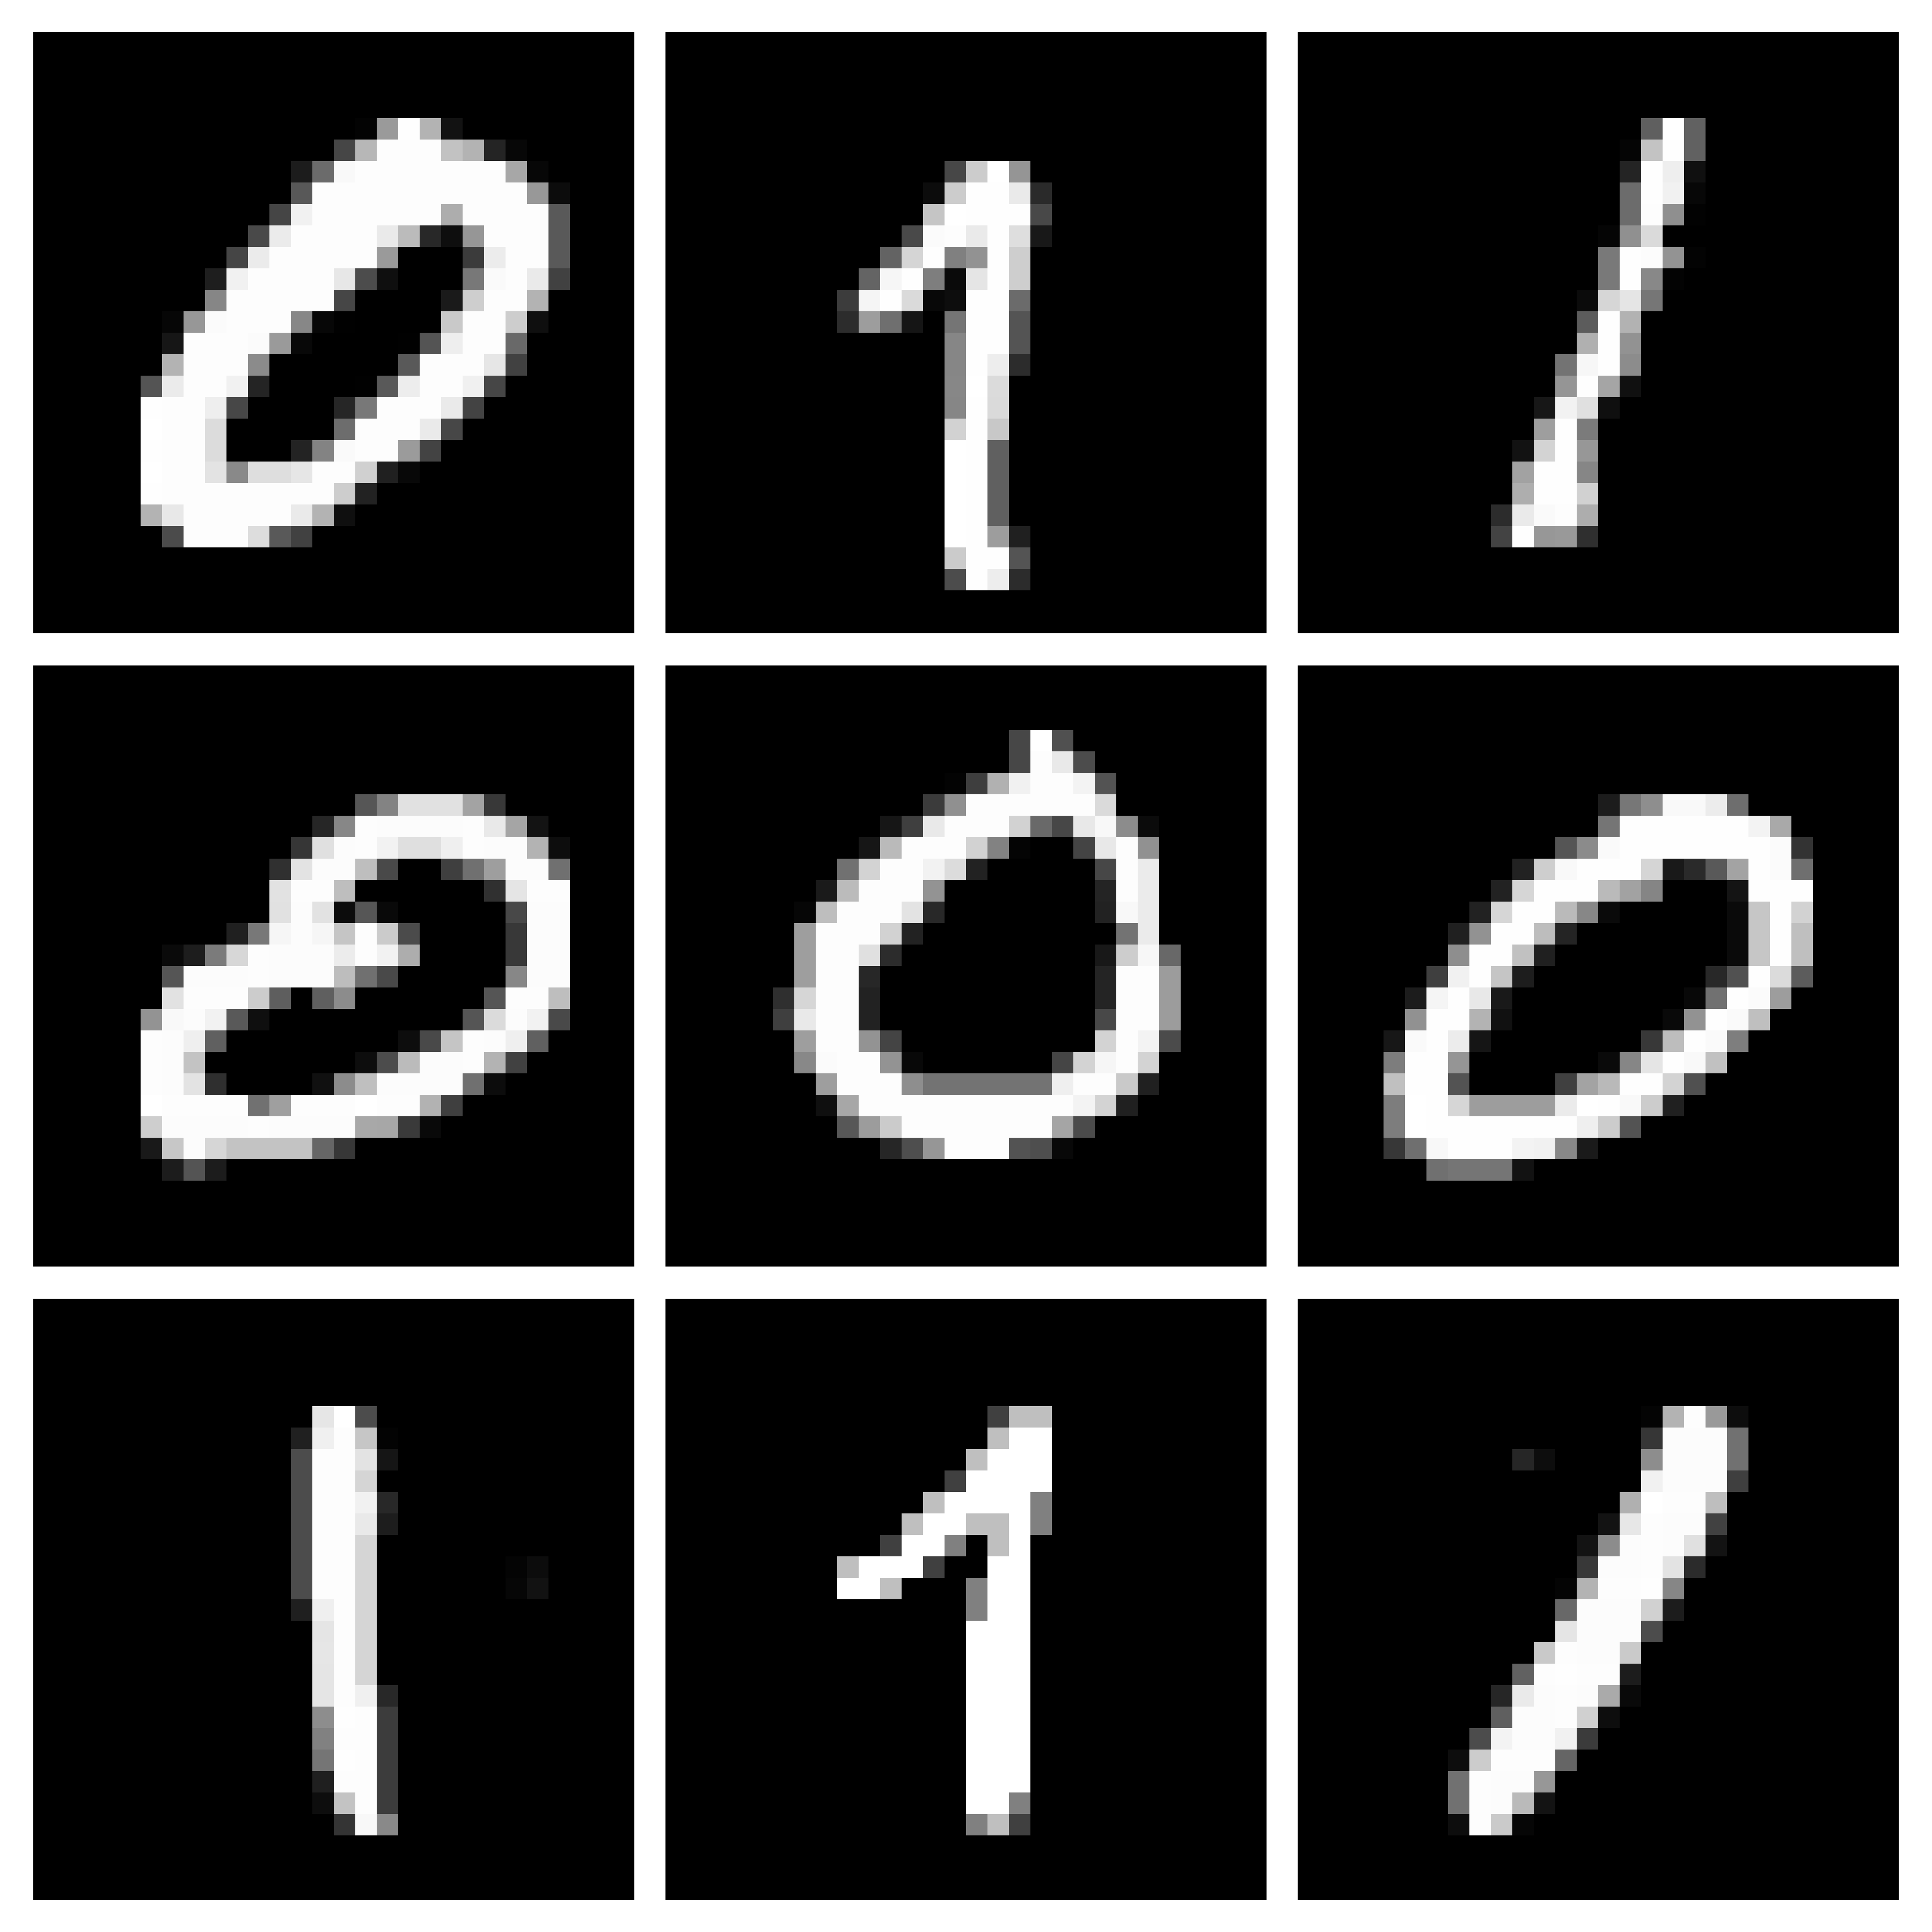
\includegraphics[width=5cm]{Graphics/mnist.png}
    \caption{Algunas imagenes contenidas en el conjunto MNIST.}
    \label{fig:mnist}
\end{figure}